\chapter{Indledning}

\section{Baggrund}
En normal synkeproces er kendetegnet ved at fødeindtagelse som passerer fra den bageste del af mundhulen, via. svælget og spiserøret til mavesækken sker uden besvær. Tilstanden hvori selve synkefunktionen og dens hastighed og frekvens forstyrres kaldes for dysfagi \cite{Sundhedsstyrelsen2015NationalDysfagi}. Dysfagi er den medicinske betegnelse for symptom relateret til synkebesvær. Der er vigtigt at differentiere mellem nedre og øvre dysfagi. Øvre dysfagi omfatter præ-oral, oral og faryngeal fase, hvorimod nedre dysfagi relaterer sig den øsefageale fase dvs. mavesæk og spiserør \cite{KjaersgaardPh.d.studerendeDYSFAGIKonsekvenser}. Det skal dog nævnes, at der er uenigheder om definitionen af dysfagi. Den manglende konsensus om definitionen gør rapportering af dysfagi insidens og prævalens uklar. Det fremgår af patientombuddets temarapport fra 2012 om dysfagi at:

\begin{itemize}
\item 60-87 \% af beboere på plejehjem for ældre har synkebesværligheder.
\item 30 \% alle apopleksipatienter har dysfagi. 15. 000 danskere rammes af hvert år af apopleksi. Forekomsten af dysfagi er ca. 37-78 \% ved akut apopleksi. Hos patienter med i den akutte fase, er dysfagi/aspiration en betydende årsag. Herudover lever 30-40.000 danskere med senfølger efter en apopleksi, nogle har dysfagi
\item 20-50 \% af patienter med Parkinson og Alzheimer har dysfagi. I 2012 havde 6. 000 patienter Parkinson og 45.000 patienter havde Alzheimer.  
\item 30-60 \% af patienter med muskelsvind har dysfagi.
\item Derudover er der ca. 10.000 børn, unge og voksne med Cerebral Parese (CP) eller kendt som "spastisk lammelse", der har synkebesvær \cite{Bommersholdt2012TemarapportDysfagi}. 
\end{itemize}

Som det ses i de nævnte statistikker, rammer dysfagi en bredt vifte af patienter fra forskellige patientgrupper. Årsagerne og konsekvenserne til dysfagi kanlæses i \nameref{bilag1}. 

\begin{figure}[H]
\centering
{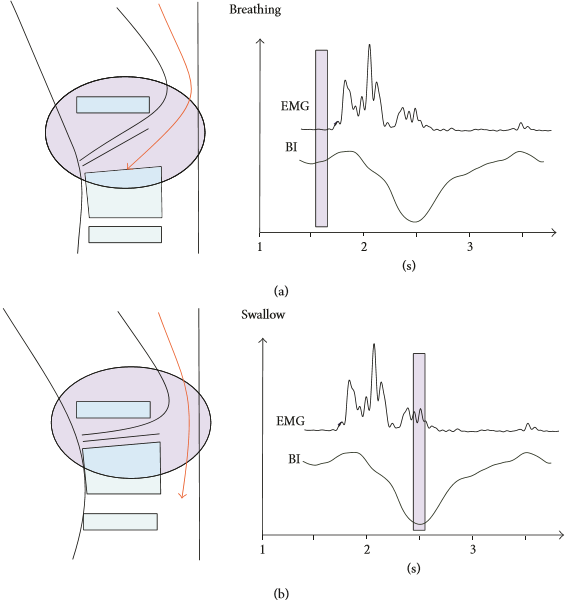
\includegraphics[width=11cm]
{Figure/EMGBIGraph}}
\caption{De tre faser ved synkeprocessen\cite{Bass1992Dysphagia:Management}}
\label{trefaser}
\end{figure}




\section{Problemformulering}